
\section{Processi primari}\label{section:Processi_primari}
\subsection{Fornitura} \label{subsection:Fornitura}
\subsubsection{Scopo}\label{subsubsection: scopo_fornitura}
In questa sezione vengono elencate tutte metriche, gli strumenti e i documenti utilizzati al fine di realizzare il processo di fornitura.
\subsubsection{Aspettative}\label{subsubsection: aspettative_fornitura}
Le aspettative nell' applicazione del processo di fornitura sono:
\begin {itemize}
    \item Avere una chiara struttura dei documenti;
    \item Definire i tempi di lavoro;
    \item Chiarire dubbi e stabilire vincoli con il proponente.
\end {itemize}
\subsubsection{Descrizione}\label{subsubsection: descrizione_fornitura}
Il processo di fornitura determina ogni compito, attività e risorsa necessaria allo svolgimento del progetto.
Tale processo verrà avviato solamente in seguito alla comprensione delle richieste del proponente, alla redazione dello \textit{studio di fattibilità} ed infine alla definizione di un accordo contrattuale con il proponente.
Il processo di fornitura consiste nelle seguenti fasi:
\begin {itemize}
    \item Avvio;
    \item Contrattazione;
    \item Pianificazione;
    \item Esecuzione e controllo;
    \item Revisione e valutazione;
    \item Consegna e completamento.
\end {itemize}
\subsubsection{Proponente}\label{subsubsection: proponente_fornitura}
Il team di sviluppo si è accordato con il proponente per avere un continuo contatto sul buon proseguo del progetto, organizzando periodicamente incontri e mantenendo un costante contatto asincrono mediante un apposito canale sulla piattaforma Discord\glo.
Il team di sviluppo vuole avere un costante contatto con il proponente riguardo alle seguenti tematiche:
\begin {itemize}
    \item Chiarimento su eventuali dubbi;
    \item Riscontro sulla documentazione redatta;
    \item Riscontro sulle tecnologie utilizzate;
    \item Opinione su soluzioni innovative proposte dal team di sviluppo
    \item Tempistiche di consegna del prodotto;
    \item Stima dei costi;
    \item Vincoli e requisiti obbligatori.
\end{itemize}
\subsubsection {Documenti}\label{subsubsection: documenti_fornitura}
Di seguito sono descritti i documenti redatti in questa fase.
\paragraph{\docNamePdQ}\label{paragraph: PdQ_fornitura}
Il \docNamePdQLow\ viene redatto dal \roleVerifierLow\ e contiene le misure necessarie a garantire la qualità del prodotto e dei processi.
Esso è formato dalle seguenti parti:
\begin{itemize}
    \item Qualità di processo;
    \item Qualità di prodotto;
    \item Specifica dei test;
    \item Resoconto attività di verifica.
\end{itemize}
\paragraph{\docNamePdP}\label{paragraph: PdP_fornitura}
Il \docNamePdPLow\ viene redatto dagli amministratori e dal \roleProjectManagerLow\ di progetto, esso verrà seguito per tutta la durata del progetto, ed è diviso nelle seguenti parti:
\begin{itemize}
    \item Analisi dei rischi;
    \item Modello di sviluppo;
    \item Pianificazione;
    \item Preventivo;
    \item Consuntivo;
    \item Organigramma;
    \item Attualizzazione dei rischi.
\end{itemize} 
\paragraph{Strumenti}\label{paragraph: strumenti_fornitura}
Di seguito sono riportati gli strumenti utilizzati dal team di sviluppo per la realizzazione del processo di fornitura:
\begin{itemize}
    \item \textbf{Microsoft Excel}: Utilizzato per creare grafici, eseguire calcoli e presentare tabelle organizzative; 
    \begin{center}
        \url{https://www.microsoft.com/it-it/microsoft-365/excel}
    \end{center}
    \item \textbf{Microsoft Project}: Utilizzato per creare i grafici di Gantt relativi alla pianificazione. 
    \begin{center}
        \url{https://www.microsoft.com/it-it/microsoft-365/project/project-management-software}
    \end{center}
\end{itemize}

\vspace{2cm}

\subsection{Sviluppo} \label{subsection:Sviluppo}
    \subsubsection{Scopo} \label{subsubsection:Sviluppo_Scopo}
    Scopo del processo di sviluppo è quello di descrivere i compiti e le attività da svolgere relative allo sviluppo del prodotto software.
    In questa sezione vengono dunque descritte le attività, le norme e le convenzioni adottate per la composizione di tale processo.

    \subsubsection{Aspettative} \label{subsubsection:Sviluppo_Aspettative}
    Le aspettative nell’applicazione del processo di sviluppo sono:
    \begin{itemize}
        \item Determinare vincoli tecnologici;
        \item Determinare gli obiettivi di sviluppo;
        \item Determinare vincoli di design;
        \item Realizzare un prodotto finale che superi i test e soddisfi requisiti e richieste del proponente.
    \end{itemize}

    \subsubsection{Descrizione} \label{subsubsection:Sviluppo_Descrizione}
    Il processo di sviluppo contiene le attività e i compiti dello sviluppatore, tra cui le attività per l’analisi dei requisiti, la progettazione, 
    la codifica, l’integrazione, il test, l’installazione e l’accettazione relative ai prodotti software.

    \subsubsection{Attività} \label{subsubsection:Attivita'}
    Di seguito sono elencate e successivamente trattate le attività caratterizzanti tale processo:
    \begin{itemize}
        \item Analisi dei requisiti;
        \item Progettazione;
        \item Codifica.
    \end{itemize}
    
        \paragraph{\docNameAdR} \label{paragraph:Analisi dei requisiti}
            \subparagraph{Scopo}
            Lo scopo dell’\docNameAdRLow\ è quello di individuare, a partire da un approfondito studio del capitolato, i requisiti diretti e indiretti,
            impliciti ed espliciti che il proponente richiede per la realizzazione del prodotto e i vari casi d'uso del prodotto stesso. In questa attività è importante
            suddividere il problema iniziale in requisiti quanto più elementari possibile, così da diminuire la complessità del problema originale
             facilitando il lavoro durante la fase di sviluppo.

            \subparagraph{Aspettative} \label{subparagraph:ADR_Aspettative}
            L’obiettivo dell’attività di \docNameAdRLow\ consiste nella creazione della documentazione formale contenente tutti i requisiti 
            richiesti dal proponente, che siano essi stati definiti all'inizio o che siano stati concordati in fase di sviluppo.

            \subparagraph{Requisiti} \label{subparagraph:Requisiti}
            I requisiti vengono raccolti da diverse fonti quali:
            \begin{itemize}
               \item Lettura investigativa del capitolato;
                \item Confronto interno tra i membri del gruppo;
                \item Confronto con il proponente;
                \item Analisi dei casi d'uso.
            \end{itemize}

            \subparagraph{Classificazione dei requisiti} \label{subparagraph:Classificazione dei requisiti}
            Ciascun requisito viene classificato mediante l'uso di un codice identificativo. Per tale codice è stato definito uno standard dal gruppo che viene spiegato nel seguito:\\\\
            \textbf{Codice Identificativo:}\\
            \begin{center}
                \textbf{\Large{R[Importanza][Tipologia][Codice]}}
            \end{center}
            dove:
            \begin{itemize}[label={}]
                \item \textbf{Importanza}: indica l'importanza associata a un requisito e può assumere un valore numerico compreso tra 1 e 3 con il seguente significato:
                
                \begin{table}[H]
                    \centering
                    \renewcommand{\arraystretch}{1.8}
                    \rowcolors{2}{green!100!black!40}{green!100!black!30}
                    \begin{tabular}{c|c}
                        \rowcolor[HTML]{125E28} 
                        \multicolumn{1}{c}{\color[HTML]{FFFFFF}\textbf{Numero}}
                        & \multicolumn{1}{c}{\color[HTML]{FFFFFF}\textbf{Descrizione}}\\
                        \hline
                        \textbf{1} & Requisito obbligatorio\\
                        \textbf{2} & Requisito desiderabile ma non obbligatorio\\
                        \textbf{3} & Requisito opzionale\\
                    \end{tabular}
                    \caption{Importanza dei requisiti}
                \end{table}
                
                \item \textbf{Tipologia}: rappresenta una tipologia di requisito e può assumere uno fra i seguenti valori letterali:
                \begin{table}[H]
                    \centering
                    \renewcommand{\arraystretch}{1.8}
                \rowcolors{2}{green!100!black!40}{green!100!black!30}
                \begin{tabular}{c|c}
                    \rowcolor[HTML]{125E28} 
                    \multicolumn{1}{c}{\color[HTML]{FFFFFF}\textbf{Sigla}}
                  & \multicolumn{1}{c}{\color[HTML]{FFFFFF}\textbf{Descrizione}}\\
                  \hline
                  \textbf{V} & Vincolo\\
                  \textbf{P} & Prestazionale\\
                  \textbf{Q} & Qualitativo\\
                  \textbf{F}  & Funzionale\\
                \end{tabular}
                \caption{Tipologie di requisiti}
            \end{table}
            \item\textbf{Codice}: è un identificativo univoco del requisito espresso in forma gerarchica padre/figlio.\\\\
        \end{itemize}
            Una volta associato a un requisito, l'identificativo è immutabile.
            Ogni requisito deve inoltre essere accompagnato da una serie di informazioni aggiuntive:
            \begin{itemize}
                \item \textbf{Descrizione}: Descrizione sintetica ed esplicativa del requisito in questione;
                \item \textbf{Classificazione}: Al fine di rendere la tabella più leggibile viene rimarcata ancora una volta l'importanza del requisito anche se già presente nel codice identificativo;
                \item \textbf{Fonte}: L'origine del requisito viene riportata in questa sezione.
            \end{itemize}
            
            \begin{table}[H]
              \centering
              \renewcommand{\arraystretch}{1.8}
              \rowcolors{2}{green!100!black!40}{green!100!black!30}
              \begin{tabular}{cccc}
                \rowcolor[HTML]{125E28} 
                \color[HTML]{FFFFFF}\textbf{Requisito}
              & \color[HTML]{FFFFFF}\textbf{Descrizione} 
              & \color[HTML]{FFFFFF}\textbf{Classificazione} 
              & \color[HTML]{FFFFFF}\textbf{Fonte}\\
            
                R1V1  &  Creazione smart contract  &  Obbligatorio  &  Capitolato C2\\    
            
              \end{tabular}
              \caption{Classificazione di un requisito}
            \end{table}
                        
            \subparagraph{Casi d'uso} \label{subparagraph:Casi d'uso}
            I casi d'uso esprimono un comportamento o un modo di utilizzare il prodotto.\\
            Vengono descritti graficamente mediante l'ausilio di diagrammi UML\glo\\
            Ciascun caso d'uso è costituito da:
            \begin{itemize}
                \item Codice identificativo;
                \item Attore Primario;
                \item Precondizioni;
                \item Postcondizioni;
                \item Scenario principale;
                \item Generalizzazioni;
                \item Estensioni.
            \end{itemize}

            \subparagraph{Classificazione dei casi d'uso} \label{subparagraph:Classificazione dei casi d'uso}
            Ciascun caso d'uso viene classificato mediante l'uso di un codice identificativo. Per tale codice è stato definito uno standard dal gruppo che viene spiegato nel seguito:\\\\
            \textbf{Codice Identificativo:}\\
            \begin{center}
                \textbf{\Large{UC[Numero caso d’uso](.[Caso d’uso figlio])* - [Titolo caso d’uso]}}
            \end{center}
            dove:
            \begin{itemize}[label={}]
                \item \textbf{UC}: Acronimo di "use case";
                \item \textbf{Numero caso d'uso}: Numero associato al caso d'uso principale;
                \item \textbf{Caso d'uso figlio}: Numero associato al sottocaso del caso d'uso principale;
                \item \textbf{Titolo caso d'uso}: Titolo assegnato al caso d'uso
            \end{itemize}

            Una volta associato a un caso d'uso, l'identificativo è immutabile.
            \begin{figure}[H]
                \centering
                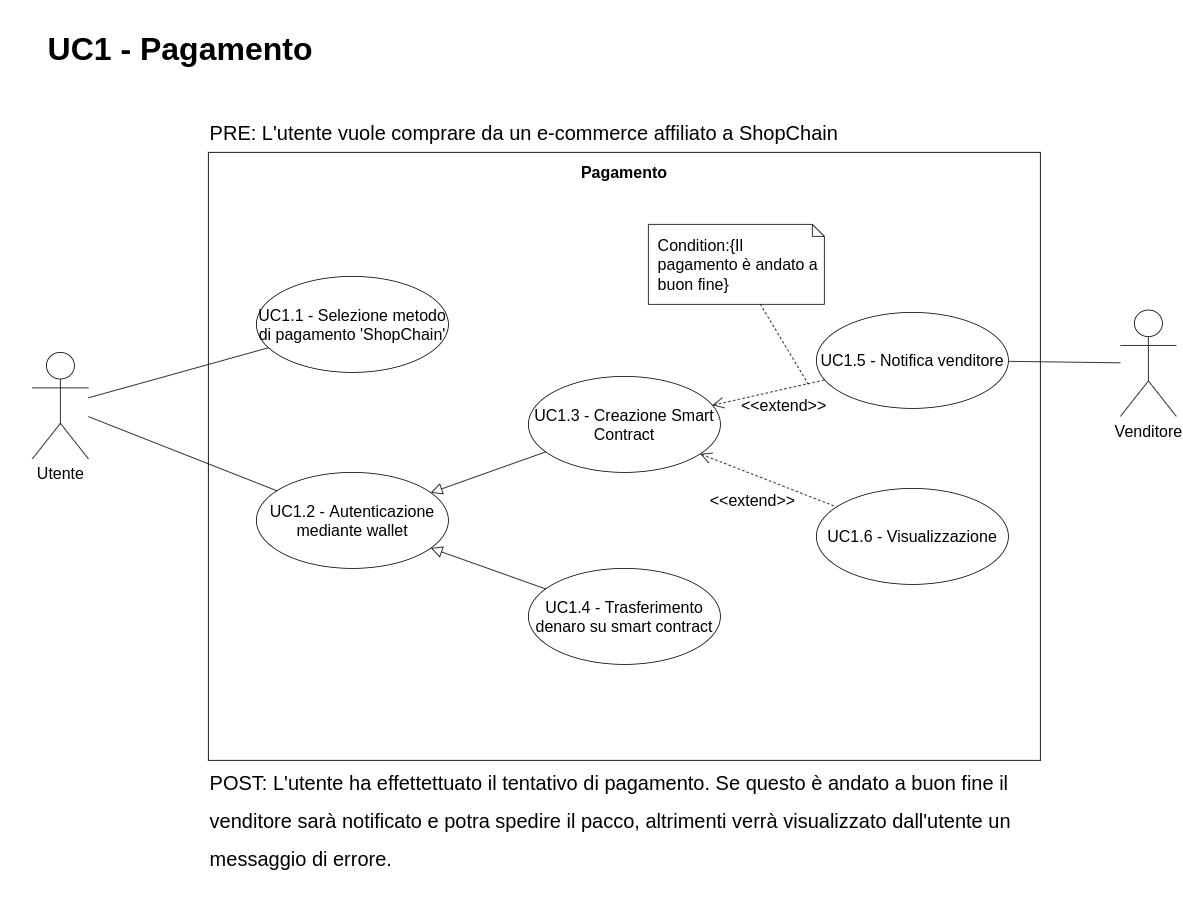
\includegraphics[scale=0.3]{../template/images/useCases/useCase.png}
                \caption{Esempio di caso d'uso}
            \end{figure}
            
            \subparagraph{UML} \label{subparagraph:UML}
            I diagrammi UML\glo\ verranno realizzati usando la versione 2.0 del linguaggio.
          
        \paragraph{Progettazione} \label{paragraph:Progettazione}

            \subparagraph{Scopo} \label{subparagraph:Progettazione_Scopo}
            Lo scopo dell'attività di progettazione è quello di incorporare le parti ottenute durante l'\docNameAdRLow, specificando le funzionalità dei sottosistemi
            e riconducendo a un’unica soluzione. 

            \subparagraph{Aspettative} \label{subparagraph:Progettazione_Aspettative}
            L’obiettivo dell’attività di progettazione consiste nel realizzare l’architettura del sistema, inizialmente realizzata da un Proof of Concept\glo\ sviluppato come
            una demo prototipale del sistema alla Requirements \& Technology Baseline, e inseguito approfondita e descritta nel documento tecnico allegato alla Product Baseline.

            \subparagraph{Requirements \& technology baseline} \label{subparagraph:Requirements & technology baseline}
            Questa fase fissa i requisiti che il fornitore si impegna a soddisfare, in accordo con il proponente e vengono motivate le tecnologie,
            i framework\glo\ e le librerie selezionate per la realizzazione del prodotto.\\
            Dimostra adeguatezza e fattibilità coerente con gli obbiettivi.\\
            Documenti utili a tali fini sono:
            \begin{itemize}
                \item \docNamePdP;
                \item \docNamePdQ;
                \item \docNameNdP;
                \item \textit{Verbali} interni ed esterni.
            \end{itemize}
            Salvo i \textit{verbali}, i documenti sopracitati vanno mantenuti ed evoluti anche per le fasi successive.\\


            \subparagraph{Product baseline} \label{subparagraph:Product baseline}
            Questa fase illustra le linee guida architetturali del prodotto.
            Oltre all'evoluzione dei documenti sopracitati, in questa fase risulteranno necessari:
            \begin{itemize}
                \item \docNameMU;
                \item \textit{Verbali di periodo}.
            \end{itemize}
            Come per la fase precedente, anche i documenti di questa fase vanno mantenuti ed evoluti fino alla fase di consegna e accettazione del prodotto finale.

        \paragraph{Codifica}    \label{paragraph:Codifica}
            \subparagraph{Scopo}    \label{subparagraph:Codifica_Scopo}
            L’attività di codifica ha il fine di concretizzare la progettazione con la programmazione del software vero e proprio.

            \subparagraph{Aspettative}    \label{subparagraph:Codifica_Aspettative}
            Questa attività dovrà avere come risultato un prodotto software avente le caratteristiche e i requisiti concordati con il proponente. Il codice generato dovrà 
            rispettare alcune norme per poter essere leggibile e per poter facilmente intervenire in seguito nelle attività di manutenzione, modifica, verifica e validazione.

            \subparagraph{Stile della codifica}    \label{subparagraph:Stile della codifica}
            \begin{itemize}
                \item \textbf{Indentazione}: I blocchi di codice innestati dovranno avere un'indentazione di quattro spazi;
                \item \textbf{Parentesi}: La parentesi aperta dovrà essere inserita nella stessa riga di dichiarazione del costrutto, separata da uno spazio, mentre
                                          la parentesi chiusa dovrà essere inserita con la giusta indentazione alla riga immediatamente successiva all'ultima riga di
                                          codice del costrutto;
                \item \textbf{Metodi}: il nome dei metodi dovrà iniziare con lettera minuscola e, se composto da più parole, le successive dovranno iniziare con lettera
                                       maiuscola. È preferibile mantenere metodi brevi, con poche righe di codice;
                \item \textbf{Classi}: il nome delle classi dovrà sempre iniziare con la lettera maiuscola e, come per i metodi, se composto da più parole, le successive 
                                       dovranno iniziare con la lettere maiuscola;
                \item \textbf{Variabili}: il nome delle variabili deve sempre essere scritto in minuscolo e in inglese. Se il nome è composta da più parole, la seconda 
                                          dovrà iniziare con la lettera maiuscola;
                \item \textbf{Costanti}: il nome deve essere sempre scritto in maiuscolo e in inglese. Se il nome è composto da più parole, queste dovranno essere separate
                                        dal carattere '\textunderscore';
                \item \textbf{Univocità dei nomi}: tutti i costrutti dovranno avere nomi univoci e significativi;
                \item \textbf{Commenti}: i commenti dovranno essere inseriti prima dell’inizio del costrutto e presentati in lingua italiana;
                \item \textbf{File}: dovranno avere un nome che inizia per lettera maiuscola che ne specifichi il contenuto.
            \end{itemize}
%%%%%%%%%%%%%%%%%%%%%%%%%%%%%%%%%%%%%%%%%%%%%
%				SISTEMARE
        \paragraph{Strumenti}    \label{paragraph:Strumenti}
        Di seguito sono riportati gli strumenti utilizzati dal team di sviluppo durante la fase di codifica e quelli utilizzati a supporto di tale processo.
        \subparagraph{Strumenti per la codifica}
        \begin{itemize}
            \item \textbf{Solidity}: È un linguaggio di programmazione orientato agli oggetti per la scrittura di smartcontract\glo . Viene utilizzato per implementare smart contract\glo\ su varie piattaforme blockchain\glo , quali ad esempio Etherium\glo , Avalanche\glo\ o Fantom\glo;
            \begin{center}\url{https://docs.soliditylang.org/}\end{center}
            \item \textbf{Remix}: È un IDE\glo\ open source\glo\ sottoforma di applicazione web e desktop che viene utilizzato per l'intero percorso di sviluppo degli smart contract\glo ;
            \begin{center}\url{https://remix.ethereum.org/}\end{center}
            \item \textbf{Truffle Suite}: 
            Truffle è un ambiente di sviluppo che consente agli utenti di testare applicazioni blockchain\glo;
            \begin{center}\url{https://trufflesuite.com/}\end{center}
            \item \textbf{Node.js}: È un runtime system\glo\ open source\glo\ multipiattaforma orientato agli eventi per l'esecuzione di codice JavaScript\glo ;
            \begin{center}\url{https://nodejs.org/it/}\end{center}
            \item \textbf{Express}: È un framework\glo\ open source\glo\ per applicazioni web per Node.js
            \begin{center}\url{https://expressjs.com/it/}\end{center}
            \item \textbf{ESLint}: È uno strumento di analisi del codice statico per identificare i modelli problematici trovati nel codice JavaScript\glo ;
            \begin{center}\url{https://eslint.org/}\end{center}
            \item \textbf{SonarCloud}: È una piattaforma per l'ispezione continua della qualità del codice per eseguire revisioni automatiche con analisi statiche del codice per rilevare bug ed errori di codice;
            \begin{center}\url{https://sonarcloud.io/}\end{center}
            \item \textbf{React}: È una libreria open source\glo , frontend\glo , JavaScript\glo\ per la creazione di interfacce utente.
            \begin{center}\url{https://it.reactjs.org/}\end{center}
        \end{itemize}
        \subparagraph{Strumenti di supporto alla codifica}
        \begin{itemize}
            \item \textbf{Docker}: Semplifica la creazione, la gestione e la distribuzione di applicazioni tramite dei contenitori, ovvero ambienti compatti (ad esempio Macchine virtuali) che forniscono una piattaforma per la compilazione e l'esecuzione di app, ma senza le dimensioni complete e il sovraccarico del sistema operativo completo.
            \begin{center}\url{https://www.docker.com/}\end{center}
            \item \textbf{Metamask}: È un'estensione browser che funge da portafoglio di criptovalute\glo. MetaMask consente ai propri utenti di conservare, scambiare e ricevere token\glo\ ETH, e più in generale tutti i token\glo\ basati sulla blockchain\glo\ Ethereum\glo ;
            \begin{center}\url{https://metamask.io/}\end{center}
            \item \textbf{Fantom testnet}: È una rete di test in cui è possibile effettuare operazioni di scambio di criptovalute\glo\ senza nessuna spesa;
            \begin{center}\url{https://docs.fantom.foundation/tutorials/set-up-metamask-testnet}\end{center}
        \end{itemize}

%%%%%%%%%%%%%%%%%%%%%%%%%%%%%%%%%%%%%%%%%%%%%